\chapter{Development follow up}
In this chapter, we will follow the development of each milestone. For each one, first, we will describe the issues involved. Then, we will describe the design decisions made, and finally, we will discuss interesting lessons and problems we have encountered in that iteration.

The Github repository used for the development of this project can be found at \href{https://github.com/salvacorts/TFG-Parasitic-Metaheuristics}{github.com/salvacorts/TFG-Parasitic-Metaheuristics}.

\section{Demo Problem}
This milestone contained the following user story:

\subsubsection*{\href{https://github.com/salvacorts/TFG-Parasitic-Metaheuristics/issues/20}{Issue \#20}: As an Administrator, I want to run a demo problem so that I can test the platform} 

Fist of all, we needed a problem that could perform well in the platform. This problem will be used to test the platform as we develop it further.

We chose a multilayer perceptron (MLP) trained with the \textit{Glass} and \textit{Cancer1a} datasets from \textit{proben1} benchmark \ref{proben1}; a set of benchmarks for neural network training algorithms.

The \textit{Glass} dataset is made of 214 samples of glass where each one contains the percent content of 8 different chemical elements, its refractive index, and the type of glass (class attribute). A model that can predict the kind of glass from new samples, can be useful in criminal forensics.

\textit{Cancer1a} is made of 699 samples of breast cancer. Each one contains a sample identification number, 9 attributes about the cell that the sample measures, and the class of cancerous cell: either benign or malignant.

There are two main reasons to have chosen a multilayer perceptron to develop and demo the platform. On the one hand, its fitness function takes more time than the average latency of communication between nodes in the platform. On the other hand, we have previous experience \ref{gprop} with this problem and we are familiar with some useful genetic operators we can apply.

The genetic operators of the genetic algorithm we have used  to optimize the neural network are the same ones proposed by P. A. Castillo et al in G-Prop \cite{gprop}:

\begin{itemize}
	\item \textbf{Selection:} Roulette tournament where two chromosomes are randomly selected from the population to cross.
	
	\item \textbf{Evaluation:} Train a copy of the chromosome with the training dataset without Backpropagation. The fitness of the chromosome that will be returned by this operator will be the classification error obtained by predicting new samples from the validation dataset with the trained copy of the chromosome.
	$$ Error = 1 - \frac{TP + TN}{TP + TN + FP + FN}  $$
	
	Where $TP = $ True Positives, $TN = $ True Negatives, $FP = $ False Positives, and $FN = $ False Negatives.
	
	\item \textbf{Mutation:} First, modify the learning rate of the network by adding a random number uniformly distributed in the range [-0.05, 0.05]. Then, with certain probability, for each neuron in each hidden layer (in our case there is just one hidden layer), add a random number in the range [-0.1, 0.1] following uniform distribution to all its weights.
	
	\item \textbf{Crossover:} Apply a multi-point crossover between two chormosomes where the neurons of both parents will be mixed resulting in two new offsprings that will contain neurons from both parents. The learning rates of the two parents are swapped as well.
	
	\item \textbf{Add Neuron:} Add a new randomly initialized neuron to the hidden layer that will be connected with the neurons in the following and previous layer. This operator performs incremental learning and attempts to address the problem of estimating the number of neurons to use in the hidden layer.
	
	\item \textbf{Eliminate Neuron:} Remove a randomly selected neuron from the hidden layer performing decremental learning. This operators aims to reduce the risks of over-fitting due to having too many neurons in the hidden layer.
	
	\item \textbf{Substitute Neuron:} Replace a random neuron from the hidden layer with a new one randomly initialized.
	
	\item \textbf{Train:} This operator performs a local search by training the multi-layer perceptron represented in the chromosome with Backpropagation \cite{backpropagation} for a given number of epochs.
\end{itemize}

We have developed our evolutionary algorithm using the \textit{Go} language \cite{go}. Go, or Golang, is a is a statically typed and compiled open-source programming language that features a C-like syntax but that includes garbage collection and easy support for concurrent and distributed programming thanks to its \textit{goroutines} \cite{channels} and \textit{channels} \cite{channels}.

There are two main pre-existing libraries that we will use:

\begin{itemize}
	\item \textbf{Go Perceptron:} A single and multilayered perceptron classifier trained with Backpropagation \cite{go-perceptron-go}.
	\item \textbf{eaopt:} An evolutionary optimization library that supports various evolutionary optimization algorithms such as genetic algorithms, particle swarm, and differential evolution among others. It also provides different genetic algorithm models, selection, mutation and crossover operators out of the box \cite{eaopt}.
\end{itemize}

\subsubsection*{Implementation}
As deliverable prototype for the end of this milestone, we wanted to have the same solution running on both native and browser environments. Typically we would have had to write the same code twice; in Go for native and in Java Script for the browser, but thanks to WebAssembly, we could share the same code base between both native and browsers with just minor changes.

The \textit{Go perceptron} library fitted our necessities well so we didn't need to modify it internally at the very first moment. On the other hand, we had to modify \textit{eopt} so we could execute other genetic operators over the population apart from the mutation, evaluation and crossover operators.

In order to use eaopt, first the developer needs to configure the number of generations, the population size and the genetic model to use in the genetic algorithm. The model defines how the algorithm evolves the population with the selection, mutation and crossover operators; in our particular case, we decided to use a generational model.

\begin{lstlisting}[
caption={eaopt's Genome interface},
label={lst:ExtraOperator}, captionpos=b]
type Genome interface {
	Evaluate() (float64, error)
	Mutate(rng *rand.Rand)
	Crossover(genome Genome, rng *rand.Rand)
	Clone() Genome
}
\end{lstlisting}

Since the implementation of these models does not contemplate additional genetic operators apart from those defined in the \textit{Genome} interface from \textit{eaopt}, we had to add an additional member to the generational model class containing an array of extra genetic operators (Listing \ref{lst:ExtraOperator}) that are used after applying mutation and crossover over a given chromosome as seen in Listing \ref{lst:opapp}.

\begin{lstlisting}[
caption={Definition of an extra genetic operator as a struct with a float representing the probability of application, and a function that takes genome and returns a modified one.},
label={lst:ExtraOperator},
captionpos=b]
type ExtraOperator struct {
	Operator    func(Genome, *rand.Rand) Genome
	Probability float64
}
\end{lstlisting}

\begin{lstlisting}[
caption={Application of extra operators after mutating.},
label={lst:opapp},
captionpos=b]
if mod.MutRate > 0 {
	offsprings.Mutate(mod.MutRate, pop.RNG)
}

for i := range offsprings {
	for _, operator := range mod.ExtraOperators {
		if operator.Probability > 0 {
			if pop.RNG.Float64() < operator.Probability {
				offsprings[i].ApplyExtraOperator(operator, pop.RNG)
			}
		}
	}
}
\end{lstlisting} 

As soon as the the genetic operators were implemented and unit tested, we proceeded to fully execute the genetic algorithm.
In order to get some insights about the state of the population during the execution of the genetic algorithm, we logged the fitness and the number of neurons of the best chromosome, and the average fitness of the population after each generation. In Figure \ref{native} we can see how the average and best fitness, as well as the number of neurons of the best solution evolves through the execution of the algorithm.

\begin{lstlisting}[
caption={Some execution logs.},
label={lst:logs},
captionpos=b]
time="2019-07-18T17:51:50+02:00" level=info msg="Best fitness at generation 0: 34.285714" Avg=65.20000000000003 Fitness=34.28571428571429 Generation=0 HiddenLayer_Neurons=16 fields.level=info
time="2019-07-18T17:51:51+02:00" level=info msg="Best fitness at generation 1: 34.285714" Avg=62.45714285714287 Fitness=34.28571428571429 Generation=1 HiddenLayer_Neurons=16 fields.level=info
time="2019-07-18T17:51:52+02:00" level=info msg="Best fitness at generation 2: 31.428571" Avg=62.342857142857135 Fitness=31.42857142857143 Generation=2 HiddenLayer_Neurons=13 fields.level=info
time="2019-07-18T17:51:53+02:00" level=info msg="Best fitness at generation 3: 25.714286" Avg=62.14285714285714 Fitness=25.714285714285708 Generation=3 HiddenLayer_Neurons=19 fields.level=info
\end{lstlisting} 

\begin{figure}[h!]
		\centering
    	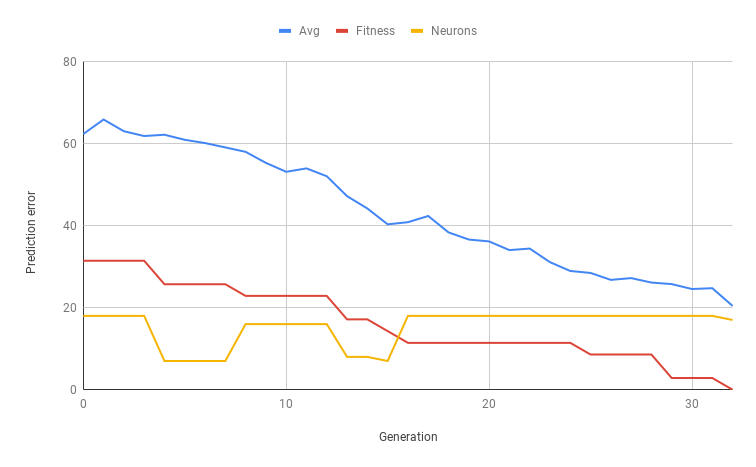
\includegraphics[width=\linewidth]{assets/images/milestone1-native-chart.png}
    	\caption{Evolution of the fitness as error predicting the validation dataset and the neural network size}
    	\label{fig:native}
\end{figure} 

We noticed that the execution of the algorithm was taking too long so we used a profiler in order to study which areas of the code were taking most of the time. It ended up being the \textit{Go perceptron} logs generator. we disabled these logs and the execution time was dramatically reduced from more than 2 hours to around 2 minutes.

Once we were pleased with the obtained results, we started to build a simple web interface as a proof of concept for the execution of the algorithm compiled into WebAssembly. We started with a very simple webpage that executed the compiled WebAssembly and displayed the logs in the console from the developers tools of the browser. But we had two problems with this approach:

On the one hand, when the browser developers tools are open, WebAssembly is actually ran like a JavaScript program in order to be able to debug it. Therefore, the execution time is considerably increased, losing the main advantage of and the reason of using WebAssembly.

As a solution, we added a HTML \textit{Div} to the webpage where we appended the logs from the program execution directly from Go using a custom class (listing \ref{lst:weblogger1}) that implemented the \textit{io.Writer} interface. By doing so, we did not need the developer tools anymore, having direct visual feedback from the execution and good performance.

\begin{lstlisting}[
caption={Weblogger class used to append logs to the webpage.},
label={lst:weblogger1},
captionpos=b]
// In main()
log.SetOutput(WebLogger{})
...

type WebLogger struct{}

func (cl WebLogger) Write(p []byte) (o int, err error) {
	logs := dom.Doc.GetElementById("logs")

	new := dom.Doc.CreateElement("p")
	new.SetTextContent(string(p))
	logs.AppendChild(new)

	return 0, nil
}
\end{lstlisting} 

On the other hand, since we were running the WebAssembly instance directly from a script imported in the HTML page, the same thread that composes the webpage is the one that executes the program and therefore, since this is a computationally intensive tasks, the browser displayed the message from figure \ref{image:kill-task} on top of the webpage. Moreover, if the user changed to another tab, the execution was paused.

\begin{figure}[h!]
		\centering
    	
\includegraphics[width=\linewidth]{assets/images/browser-warning.png}
    	\caption{Browser warning about computationally intensive tasks}
    	\label{image:kill-task}
\end{figure} 

We solved this by using a webworker \cite{webworker}; a script that runs in a separate thread in the background. The problem with webworkers is that they do not have access to the DOM, instead, they have to communicate with another thread that is being executed in the browser's main thread. It is a simple but limited API where the main thread launches the worker and sets an event listener for incoming messages. Then the worker posts a new message as a string that is delivered to the main thread. Figure \ref{logging-system} illustrates the webworker behaviour we used for the logging system.

\begin{figure}[h!]
		\centering
    	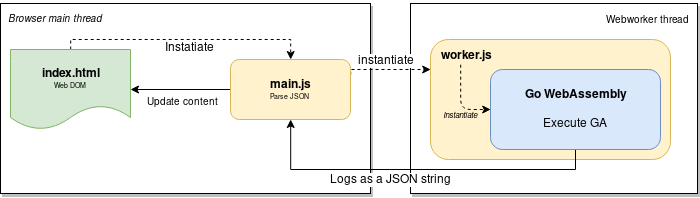
\includegraphics[width=\linewidth]{assets/images/logging-system.png}
    	\caption{The \textit{main.js} script loaded in the main HTML document, starts a webworker that will start the webassembly runtime and load the compiled Go program into it. The logs generated in Go are received by the main thread through the webworker API and these are appended into the web DOM}
    	\label{image:logging-system}
\end{figure} 

Since now we had a background job doing the most demanding work, the main thread was free to compose the webpage so we added two line charts using \textit{chart JS} to display live information about the execution. In order to parse the information needed to compose the charts from the logs, we changed their format to JSON in order to deserialize them to Java Script objects and access their information faster and easier.

This concludes the first milestone in the project. The deliverable prototype is the resulting web interface for the genetic algortihm that trains the multi layer perceptron in WebAssembly. It can be found at \href{https://salvacorts.github.io/TFG-Parasitic-Metaheuristics/mlp-ea/web/src/}{salvacorts.github.io/TFG-Parasitic-Metaheuristics/mlp-ea/web/src/} and looks as follows.

\begin{figure}[h!]
		\centering
    	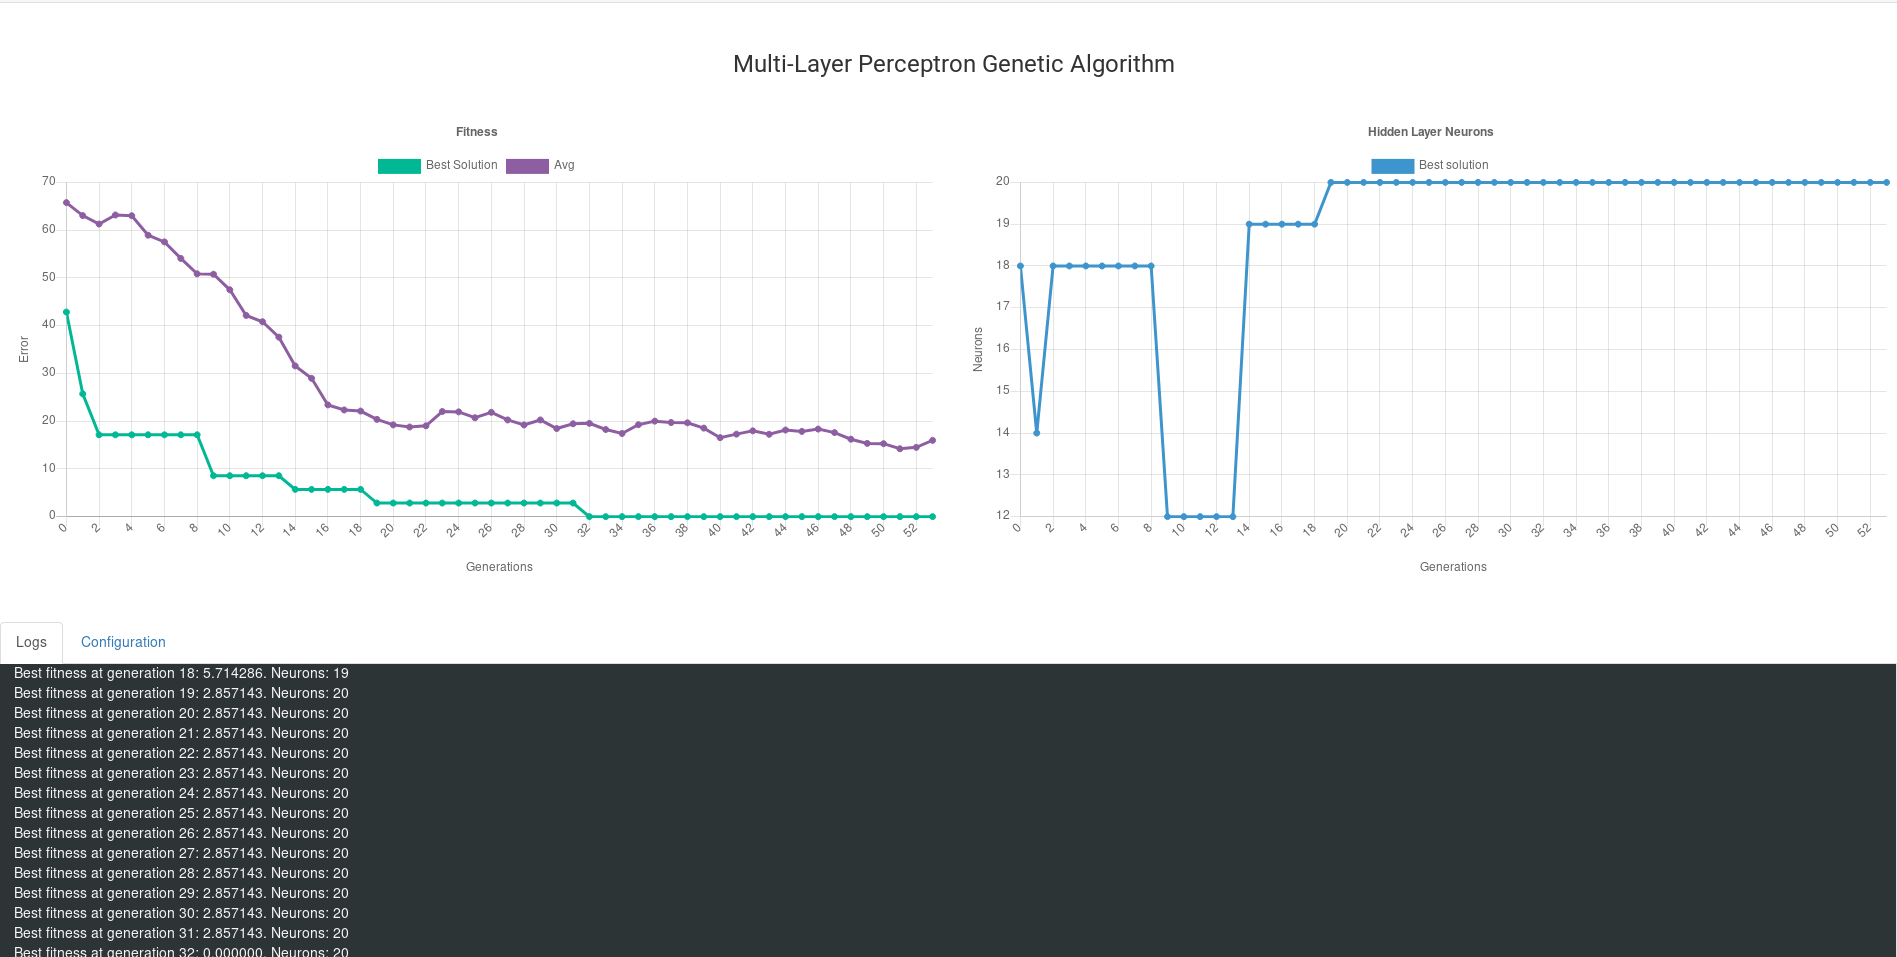
\includegraphics[width=\linewidth]{assets/images/web-milestone1.png}
    	\caption{Final prototype of the webpage running the Go code for the genetic algorithm in webassembly.}
    	\label{image:web-milestone1}
\end{figure}

The genetic algorithm implementation can be found in the main repository in directory \textit{mlp-ea/common}. The web source can be found in \textit{mlp-ea/web}. The source of the program to execute it natively can be found in \textit{mlp-ea/native} and can be directly run as in Listing \ref{lst:run} or compiled and run as in \ref{lst:build-run}.

\begin{lstlisting}[
caption={Run native program},
label={lst:run},
captionpos=b]
go run main.go
\end{lstlisting} 

\begin{lstlisting}[
caption={Build program and run},
label={lst:build-run},
captionpos=b]
go build main.go
./main
\end{lstlisting} 


\section{Centralized Distributed Evolutionary Algorithm}

In this milestone we aimed to develop a distributed evolutionary algorithm with a client server architecture to solve our MLP problem developed in the previous milestone.

\subsubsection*{\href{https://github.com/salvacorts/TFG-Parasitic-Metaheuristics/issues/9}{Issue \#9}: As a researcher, I want different systems to communicate between each others with a common solution representation so that all of them can work with it and share it.}

Both clients and server need to communicate with each other to work together, to do so, we need to provide a common data representation that enables them to work and exchange chromosomes over the internet. 

We chose Protocol Buffers as our serialization and data definition mechanism since, as we previously saw in chapter 3, it is a simple, fast and extensible solution that outperforms the most commonly used data representation techniques like XML or JSON, and supports many languages which makes it a really attractive alternative for future support for other languages apart from Go.

Moreover, we decided to use \textit{gogoprotobuf} \cite{gogo}, a fork of Protocol Buffers for Golang that comes with important optimization and extra features. Several benchmarks \cite{gogo-bench} comparing this fork with the rest of serialization and deserialization solutions for Golang demonstrates that \textit{gogoprotobuf} is the best choice in terms of performance, correctness, and interoperability.

In Listing \ref{lst:mlp-protobuf} we can find the protocol buffers representation for the Multilayer Perceptron we used in the previous milestone. Once this type is compiled into Golang, its usage slightly differs from a traditional Go type, therefore, we had to adapt all our mlp-related functions from \textit{go-perceptron-go} to work with this new type; including the training and prediction methods, as well as all the genetic operators.

\begin{lstlisting}[
language=protobuf2,
caption={Protocol Buffers representation of the Multilayer Perceptron},
label={lst:mlp-protobuf},
captionpos=b]
enum TransferFunc {
    SIGMOIDAL = 0;
}

message NeuronUnit {
    repeated double Weights = 1;
    double Bias = 2;
    double Lrate = 3;
    double Value = 4;
    double Delta = 5;
}

message NeuralLayer {
    repeated NeuronUnit NeuronUnits = 1 [(gogoproto.nullable) = false];
    int64 Length = 2;
}

message MultiLayerNetwork {
    double LRate = 1;
    repeated NeuralLayer NeuralLayers = 2 [(gogoproto.nullable) = false];
    TransferFunc TFunc = 3;
}
\end{lstlisting} 

In order to test that this new Protocol Buffers type and the modified functions were behaving as expected, we used the same unit tests we were using for the genetic algorithm using \textit{go-perceptron-go} in the previous iteration to validate our new implementation. We achieved the same performance and results as on the previous milestone.

\subsubsection*{\href{https://github.com/salvacorts/TFG-Parasitic-Metaheuristics/issues/21}{Issue \#21}: As a researcher, I want an interface for browser-based nodes communications so that using the distributed system is easier.}

If two collaborating nodes want to communicate with each other, they would have to enable port-forwarding on their local gateways. Since this project aims to achieve minimal installation requirements, and most routers provided by ISPs do not provide any mechanism to open ports in the router from inside an application (e.g. \textit{UPnP} \cite{wiki-upnp} is missing or deactivated in most cases) without the explicit intervention of the user for security reasons, we need to rely on a central server that will take the role of intermediaries between clients.

We have based our design on the pool-based genetic algorithm from Merelo et al \cite{paper-pool-jj} where the central server maintains a pool of chromosomes that are mutated and crossed by the server and evaluated by the clients.

Although in \cite{paper-pool-jj} the pool of chromosomes that is modified by the server is implemented using the NoSQL database CouchDB, we thought that this leads to an avoidable extra time to process modification requests on the database and memory overhead consumption. So that, we used \textit{go-cache} \cite{go-cache} instead, an in-memory cache that is fast and thread-safe by only locking the index that is being modified instead of the entire data structure when a write occurs.

The server uses four threads to manipulate the population, each thread is in charge of an specific task:

\paragraph*{MainThread.} It is in charge of randomly initializing the population at the beginning of the algorithm execution, selecting chromosomes, crossing the selected ones, mutating them and applying the extra genetic operators from the previous milestone.

The selection operator differs from the one used in the first milestone in order to increase exploitation capabilities since a roulette selection led us to poor results on this architecture due to the lack of convergence in the population. We used a selection mechanism where 4 offspring are selected after each one wins a tournament of 4 candidates randomly picked from the population.

A chromosome $A$ is better candidate than a chromosome $B$ if the fitness of $A$, rounded to 2 decimals, is lower than the fitness of $B$, and in case both finesses are equal, $A$ has less neurons in total than $B$.

Once an individual is modified or newly generated by crossover, it is no longer evaluated and therefore it is removed from the population and appended into the evaluation channel that communicates this thread with the \textit{Evaluate handler} thread.

\paragraph*{Population growth control.} Since the crossover population creates new chromosomes that are evaluated and appended to the population, it can grow out of proportion. To avoid this scenario, the \textit{population growth control} thread periodically reduces the population to the initial population size by removing the less fit individuals. Also, to increase convergence, the worst individual from the remaining population is replaced by the best solution found so far.
	
\paragraph*{Evaluate handler.} Creates a new gRPC server that listens for requests from clients asking for new individuals to evaluate, or returning evaluated ones. 

In \cite{paper-pool-jj}, this was done with a RESTful API that used HTTP 1.0 as transport protocol and JSON as data representation schema. Instead, we have chosen gRPC \cite{grpc} to provide an interface for communication between clients and the server.

\begin{lstlisting}[
language=protobuf2,
caption={Protocol Buffers definition of our gRPC service for the evaluation of chromosomes},
label={lst:grpc-protobuf},
captionpos=b]
message MLPMsg {
    MultiLayerNetwork mlp = 1;
    string individualID = 2;
    bool evaluated = 3;
    double Fitness = 4;
    string clientID = 5;
}

message ProblemDescription {
    string clientID = 1;
    int64 epochs = 2;
    int64 folds = 3;
    string trainDataset = 4;
    repeated string classes = 5;
}

service DistributedEA {
    rpc GetProblemDescription(google.protobuf.Empty) returns (ProblemDescription) {}
    rpc BorrowIndividual(google.protobuf.Empty) returns (MLPMsg) {}
    rpc ReturnIndividual(MLPMsg) returns (google.protobuf.Empty) {}
}
\end{lstlisting}

On the one hand, gRPC services are defined with protocol buffers which made it easier for us to implement this service given our previous design decisions. It also reduces the latency between peers since, as stated on previous sections, the serialization and deserialization times and sizes for Protocol Buffers are much lower than for JSON.

On the other hand, gRPC uses HTTP/2, an evolution of HTTP 1.1, that provides request multiplexing and header compression. In order to demonstrate its capabilities, we have modified an Open Source benchmark \cite{rest-vs-grpc-bench} written in Go that compares the performance of gRPC vs REST by requesting and serving the same object multiple times. The original version of this benchmark served a small object made of just a couple of small fields. In order to better fit our scenario, we have modified this object (Listing \ref{lst:bench-struct}) to have a payload made of an array of 64 bit floats and 10000 elements.

\begin{lstlisting}[
caption={Response object used for the benchmark},
label={lst:bench-struct},
captionpos=b]
type Response struct {
	Message string    `json:"message"`
	Code    int       `json:"code"`
	User    *User     `json:"user"`
	Payload []float64 `json:"payload"`
}

func fillPayload() []float64 {
	payload := make([]float64, 10000)
	for i := range payload {
		payload[i] = 0.0
	}

	return payload
}
\end{lstlisting}

As it can be seen on Listing \ref{lst:grpc-vs-rest} and Figure \ref{fig:grpc-vs-rest} , the response time of the gRPC server is an order of magnitude faster than the REST server. Moreover, it also has smaller memory impact; consuming  28\% less RAM and performing 35 less allocations per iteration. 

\begin{lstlisting}[
language=bash,
caption={gRPC using HTTP2.0 and Protocol Buffers performance vs REST using HTTP 1.1 and JSON },
label={lst:grpc-vs-rest},
captionpos=b]
goos: linux
goarch: amd64
pkg: github.com/plutov/benchmark-grpc-protobuf-vs-http-json
Benchmark`\textcolor{red}{GRPCProtobuf}`-12            2000            `\colorbox{yellow}{527570 ns/op}`          395390 B/op        223 allocs/op
Benchmark`\textcolor{red}{HTTPJSON}`-12                 200           `\colorbox{yellow}{7523902 ns/op}`          554060 B/op        258 allocs/op
PASS
ok      github.com/plutov/benchmark-grpc-protobuf-vs-http-json  5.313s
\end{lstlisting}

\begin{figure}[h!]
        \centering
        \begin{subfigure}{.5\textwidth}
          \centering
          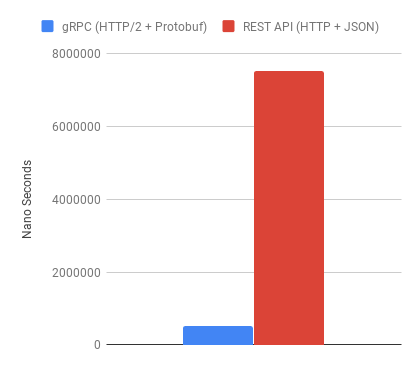
\includegraphics[width=\linewidth]{assets/images/grpc-vs-rest-time.png}
          \caption{Latency}
        \end{subfigure}%
        \begin{subfigure}{.5\textwidth}
          \centering
          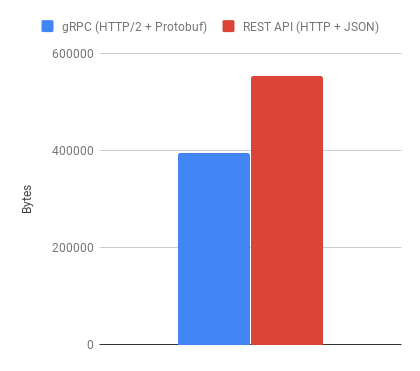
\includegraphics[width=\linewidth]{assets/images/grpc-vs-rest-memory.png}
          \caption{Memory usage}
        \end{subfigure}
        \caption{Performance of gRPC (blue) vs REST API (red). Less is better}
        \label{fig:grpc-vs-rest}
    \end{figure}
    
It is worth mentioning that as of August 11th, there is no current official support for gRPC on Golang Web Assembly although it is in process \cite{grpc-wasm-issue}. As a workaround, we are setting two listeners for the gRPC server: a \textit{tcp} listener for native clients that will support HTTP/2, and a \textit{Web Sockets} listener for Web Assembly clients that will work on top of HTTP 1.1. Still, we take advantage of the benefits of using Protocol Buffers over JSON.

\paragraph*{Evaluated handler.} When the gRPC server gets back an individual from a client, it appends that individual into the evaluated channel which connects the \textit{Evaluate handler} thread with the \textit{Evaluated handler} thread which is in charge of appending the received individuals into the population. It is also responsible for checking if the received solution is better than the best one so far, or if the stopping criteria is met. In our case, the stopping criteria are either reaching a maximum number of evaluations or the best solution having a fitness of 0.0.

\paragraph*{}
The resulting prototype for this milestone is a working distributed evolutionary algorithm that can be found at \href{github.com/salvacorts/TFG-Parasitic-Metaheuristics/tree/master/mlp-ea-centralized/common}{https://github.com/salvacorts/TFG-Parasitic-Metaheuristics/tree/master/mlp-ea-centralized/}, and executed as follows:

\begin{itemize}
	\item \textbf{Server.} Listens at 127.0.0.1:3117.
\begin{lstlisting}[language=bash]
cd native/server/
go run server.go
\end{lstlisting}

	\item \textbf{Native Client.} Can be instanced multiple times by running the following command as many times as desired.
\begin{lstlisting}[language=bash]
cd native/client/
go run client.go
\end{lstlisting}

	\item \textbf{Web Client.} Can be instance in multiple tabs by running the instructions bellow and opening \href{127.0.0.1:8081}{127.0.0.1:8081} in a browser.
\begin{lstlisting}[language=bash]
fab build-web-mlp-wasm
fab run-server-web-mlp
\end{lstlisting}
\end{itemize}

\begin{figure}[h!]
		\centering
    	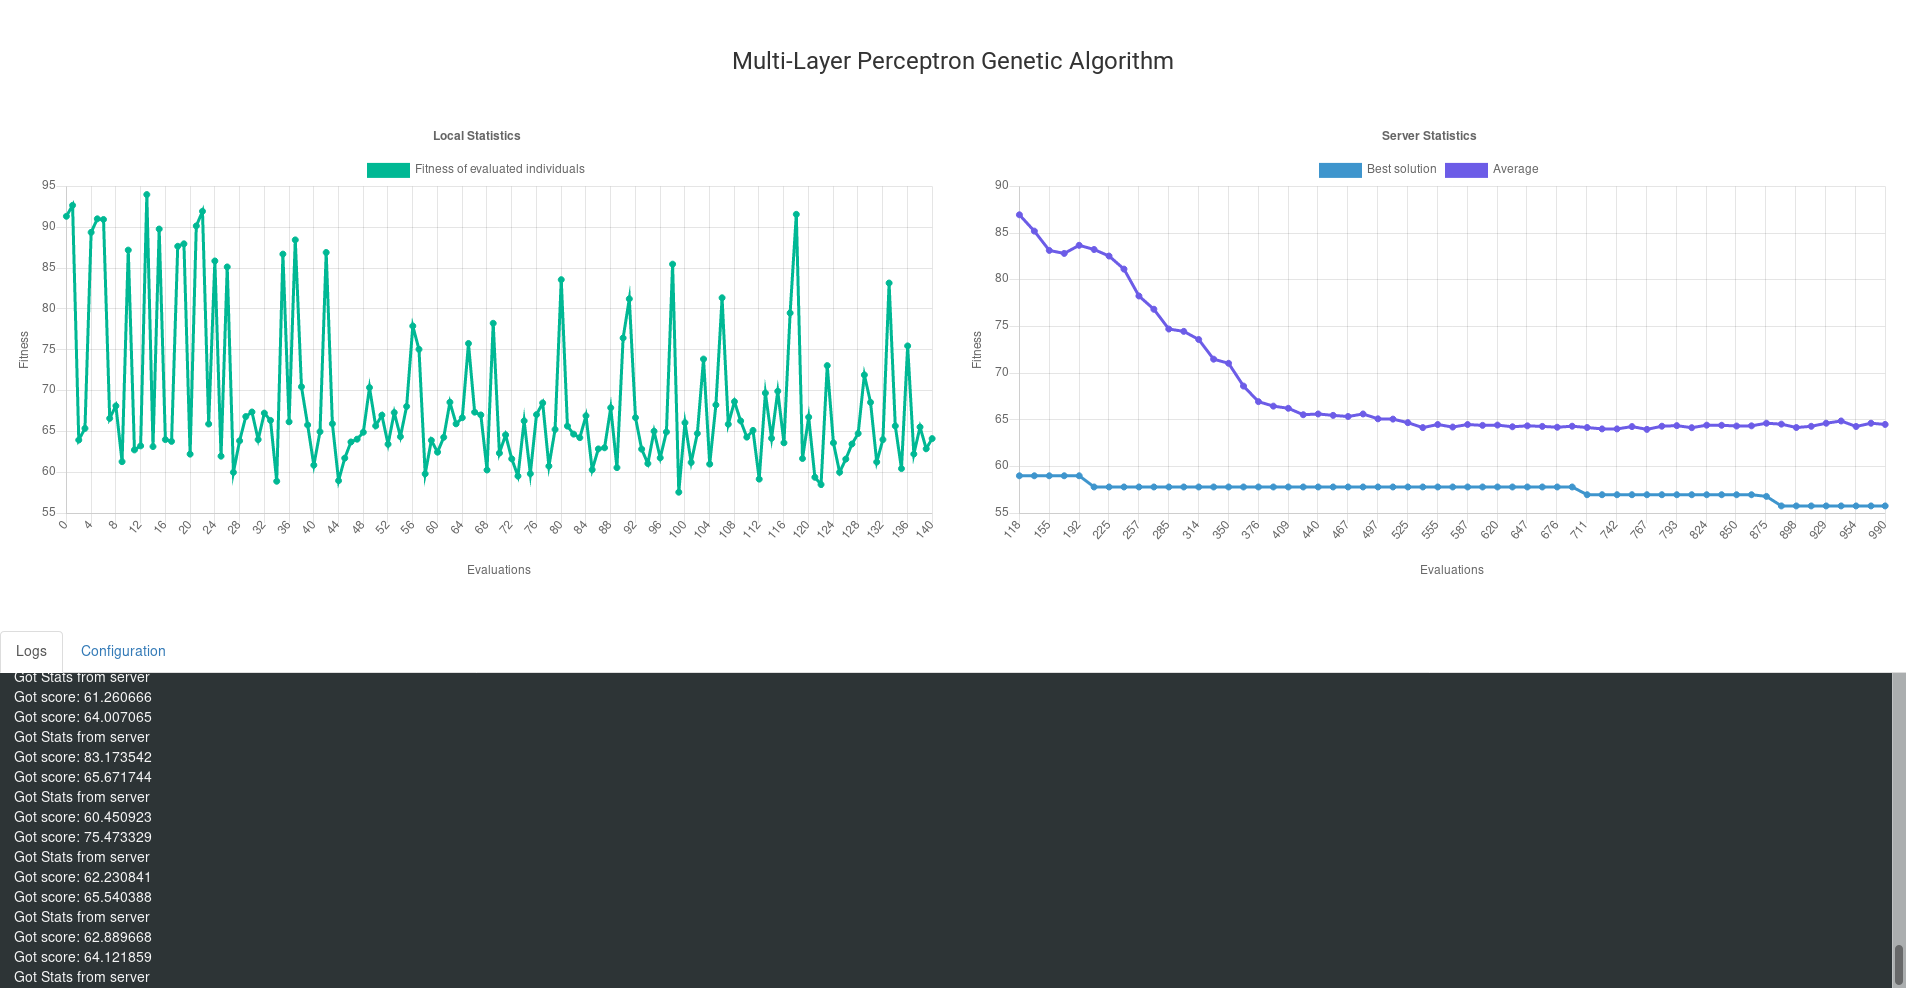
\includegraphics[width=\linewidth]{assets/images/web-milestone2.png}
    	\caption{Final prototype of the webpage running the Go code that evaluates individuals from the server.}
    	\label{image:web-milestone2}
\end{figure}

\section{Decentralized Distributed Evolutionary Algorithm}

The objective for this milestone was to decentralized the implementation from the previous milestone as well as providing more metrics to better assess the execution of the algorithm in a cluster of nodes. This sprint contained the user stories described bellow.

\subsubsection*{\href{https://github.com/salvacorts/TFG-Parasitic-Metaheuristics/issues/18}{Issue \#18}: As a researcher, I want an interface for native nodes communications so that using the distributed system is easier.}
So far our algorithm was tightly coupled to our testing problem, so that, the first objective of this story was to decouple the problem from the algorithm itself.

Since our RPC service was defined using the configuration fields for the MLP execution, and the \textit{MultiLayerNetwork} type from the MLP problem, we had to redefine the service messages, as in Listing \ref{lst:rpc_milestone3}, using an array of bytes as the payload for the genome and the problem description instead of using the problem specific types as in Listing \ref{lst:grpc-protobuf}.

\begin{lstlisting}[
language=protobuf3,
caption={Modified gRPC service to be decoupled from the problem by using an array of bytes to define the genome of an Individual and the problem description. Changes with respect to the types of the previous iteration are highlighted}.,
label={lst:rpc_milestone3},
captionpos=b]
message `\colorbox{yellow}{Individual}` {
    string individualID = 2;
    bool evaluated = 3;
    double fitness = 4;
    `\colorbox{yellow}{bytes genome = 5;}`
}

message ProblemDescription {
    string clientID = 1;
    `\colorbox{yellow}{bytes payload = 2;}`
}

service DistributedEA {
    rpc GetProblemDescription(google.protobuf.Empty) returns (`\colorbox{yellow}{ProblemDescription}`) {}
    rpc BorrowIndividual(google.protobuf.Empty) returns (`\colorbox{yellow}{Individual}`) {}
    rpc ReturnIndividual(`\colorbox{yellow}{Individual}`) returns (google.protobuf.Empty) {}
}
\end{lstlisting}

The implementation of this service had to be modified as well since we no longer had direct access to the actual representation of the genome nor the problem description. We solved this by using a similar approach as to abstract the actual genetic operators implementations from the algorithm: a delegate interface (Listing \ref{lst:delegate_interface}) to be implemented by the user to serialize and deserialize the genome of an Individual and the problem description.

\begin{lstlisting}[
caption={Delegate interface to be implemented by the user that enables the algorithm to serialize and deserialize the genome and problem description.},
label={lst:delegate_interface},
captionpos=b]
type ServiceDelegate interface {
	SerializeProblemDescription() []byte
	DeserializeProblemDescription([]byte)
	SerializeGenome(eaopt.Genome) []byte
	DeserializeGenome([]byte) eaopt.Genome
}
\end{lstlisting}

The implementation of this interface for the user should be trivial. For example, the \textit{DeserializeProblemDescription} and \textit{SerializeGenome} functions for the MLP problem looks as in Listing \ref{lst:mlp_delegate}

\begin{lstlisting}[
caption={Delegate interface implementation for the MLP problem.},
label={lst:mlp_delegate},
captionpos=b]
// DeserializeProblemDescription sets mlp.Config from deserializing buff
func (d DelegateImpl) DeserializeProblemDescription(buff []byte) {
	desc := MLPDescription{}

	err := desc.Unmarshal(buff)
	if err != nil {
		Log.Fatalf("Could not deserialize MLPDespription. %s", err.Error())
	}

	Config.Epochs = int(desc.Epochs)
	Config.Folds = int(desc.Folds)
	Config.Classes = desc.Classes

	Config.TrainingSet, err, _ = utils.LoadPatternsFromCSV(desc.TrainDataset)
	if err != nil {
		Log.Fatalf("Could not Parse patterns from reterived CSV. %s", err.Error())
	}
}

// SerializeGenome serializes a MLP to a []byte
func (d DelegateImpl) SerializeGenome(genome eaopt.Genome) []byte {
	mlp := genome.(*MultiLayerNetwork)

	buff, err := mlp.Marshal()
	if err != nil {
		Log.Fatalf("Could not serialize MultiLayerNetwork. %s", err.Error())
	}

	return buff
}
\end{lstlisting}

With these changes, we had a library to execute distributed genetic algorithms that does not depend on the problem description nor solution representation.

\paragraph*{}
The second and main objective of this story was to shift from a centralized network toward a peer-to-peer network design.
All distributed systems needs from mechanisms to keep track of other nodes in the system; this is easily achievable in a centralized approach since all nodes need to know only about the central node that coordinates them, but it is much more complicated on decentralized networks since each node needs to maintain a list of alive nodes and look for failures on other nodes of the network by its own.

We used a Gossip protocol to implement the membership and failure detection mechanism of our decentralized network. Gossip protocols spread information though a network in a similar way to how a gossip, or an infection, is spread in society. They are widely used in the industry to achieve this; an example of a successful product that makes use of a Gossip protocol to achieve the same goal as us is Amazon's Dynamo Database\cite{dynamo_paper}; a scalable and decentralized NoSQL database capable of serving more than 10 trillion requests per day and support above 20 million requests per second \cite{dynamo_web}.

Specifically, the Gossip protocol we used to build our system is the SWIM membership protocol\cite{SWIM} by using the Go \textit{memberlist} library\cite{memberlist}. The SWIM protocol has two components that work as follows\cite{SWIM}:

\paragraph*{Failure Detector.} In order to detect failing nodes in the system, a node $M_{i}$ from the cluster periodically sends a ping to a randomly selected node $M_{j}$ from its list of nodes. If $M_{j}$ does not answer back within a given timeout based on the round-trip time of the message, $M_i$ selects $k$ nodes from its list of nodes and requests each one to ping $M_j$. If $M_{j}$ answers back to any of the selected $k$ nodes, the ping response will be forwarded to $M_{i}$. At the end of the given protocol period ($T'$), $M_{i}$ checks whether an ping response was received or forwarded from $M_J$; if not, $M_{j}$ marked as \textit{Suspected} of failing in $M_{i}$'s members list.

\begin{figure}[h!]
		\centering
    	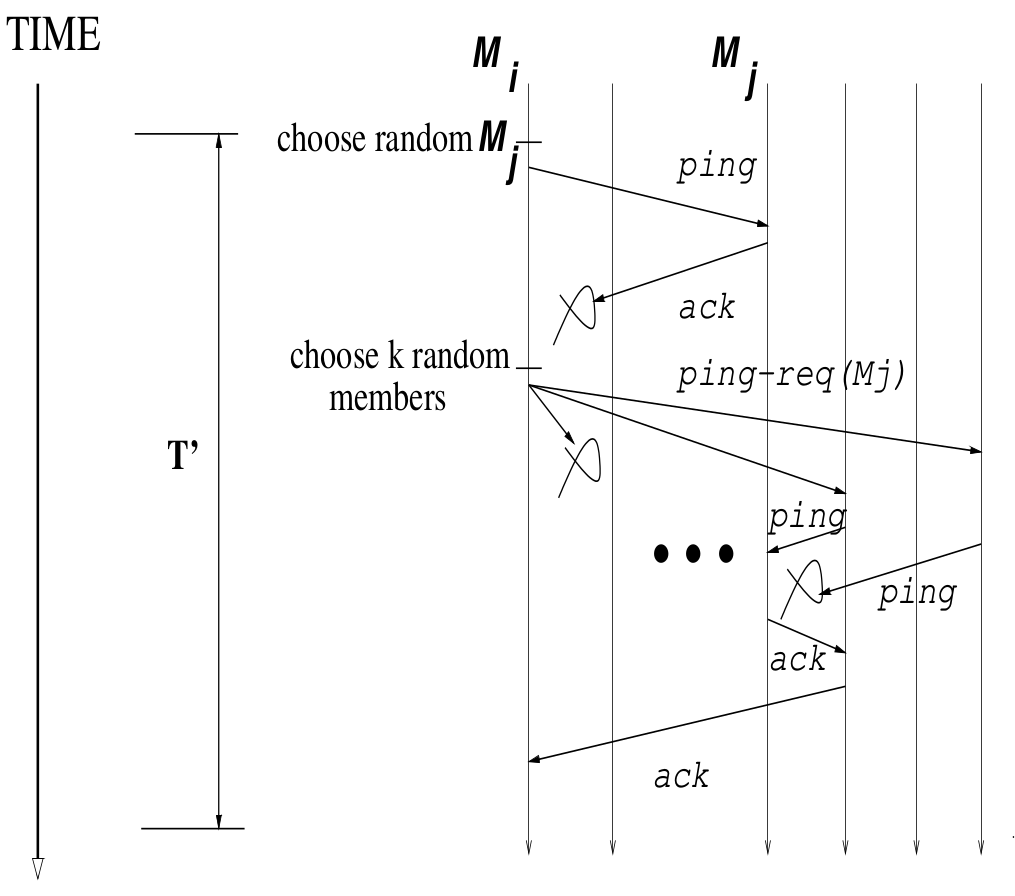
\includegraphics[scale=0.25]{assets/images/swim_net.png}
    	\caption{SWIM mechanism for node failure detection. $M_{i}$ request $k$ nodes from the cluster to ping $M_{j}$ and forward its response back after not receiving an response back to $M_{i}$'s original ping. \cite{SWIM}}
    	\label{image:web-milestone2}
\end{figure}

Then, using the Dissemination Component, a message \textit{\{Suspect $M_{j}$: $M_{i}$ suspects $M_{j}$\}} is spread through the system and nodes that receive that message will mark $M_{j}$ as \textit{Suspected}. If a node $M_{l}$ that has marked $M_{j}$ as \textit{Suspected} does not receive an \textit{Alive} message about $M_{j}$ before a given timeout, $M_{l}$ will remove $M_{j}$ from its list of members declaring it as faulty and spread the message \textit{\{Confirm $M_{j}$: $M_{l}$ declares $M_{j}$ as faulty\}} thought the Dissemination Component.\cite{SWIM}

\paragraph*{Dissemination Component.} Gossiping is done by piggybacking messages on the requests and responses from the Failure Detector component.

From \cite{epidemics}, for a cluster of $n$ nodes, the relation between the expected number of infected members $x$ and time $t$, with a contact rate $\beta$ per time unit is obtained as equation \ref{eq:2}.
\begin{equation}
\label{eq:2}
    \frac{dx}{dt} = \beta \cdot x \cdot (n - x)
\end{equation}

For SWIM, having $T'$ as time unit and the probability of contacting a node from another node's members list as $\beta$; the above equation leads to equation \ref{eq:3}.
\begin{equation}
\label{eq:3}
   x = \frac{n}{1 + (n - 1)e^{-(2- \frac{1}{n})t}}
\end{equation}

Each message will be piggybacked at most $\lambda \cdot \log n$ times (where $\lambda$ is a given constant), since that message will be spread to $ x = \frac{n}{1 + (n - 1)e^{-(2-1/n)\lambda}} \ge n \cdot (1 - \frac{1}{n^{(2-1/n)\lambda-1}}) $ members after $\lambda \cdot \log n$ protocol periods. The least gossiped messages have higher priority.

All in all, as the number of nodes in the cluster increases ($n \rightarrow \inf$), the number of nodes to contact, $x$, goes to $(n - n^{-(2\lambda - 2)})$\cite{SWIM}. So the parameter $\lambda$ enables the user to adjust the gossip protocol reliability; a smaller $\lambda$ leads to lower reliability but with lower bandwidth usage, whereas a higher $\lambda$ increases reliability at cost of bandwidth.

\begin{figure}[h!]
		\centering
    	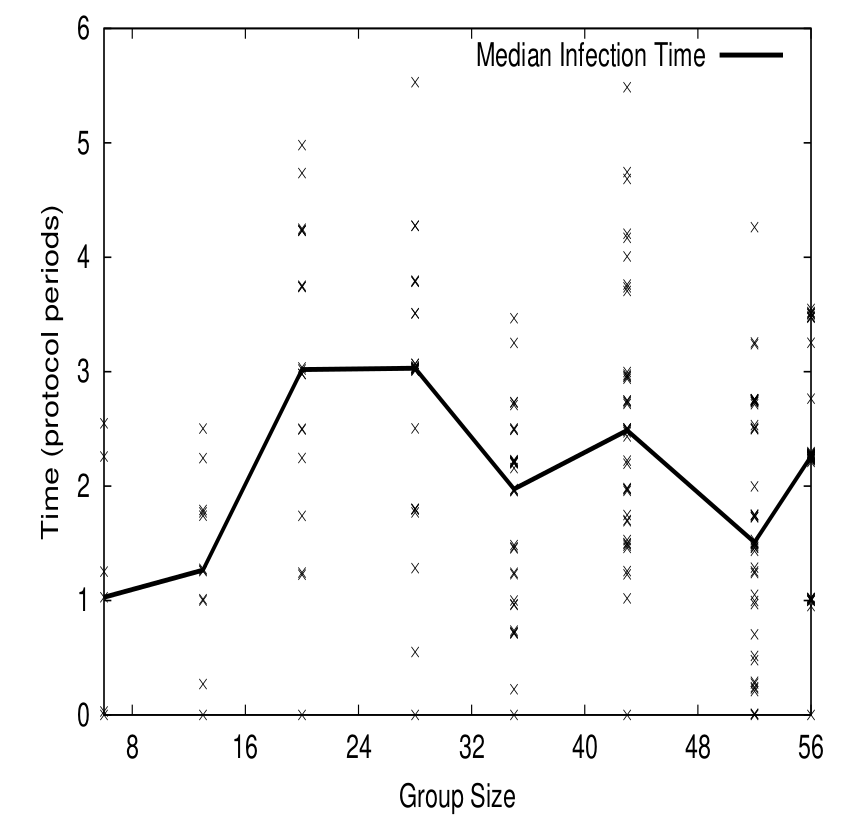
\includegraphics[scale=0.25]{assets/images/swim_chart.png}
    	\caption{Message spead latency variation with cluster size. \cite{SWIM}}
    	\label{image:web-milestone2}
\end{figure}

In our system, apart from using the SWIM protocol to maintain nodes membership, we used the Dissemination Component to spread newly found best individuals across the system so every node in the cluster knows the best individual found so far with eventual consistency as a way to increase the exploitation capabilities of the evolutionary algorithm. Also, with every \textit{Alive} message, metadata about the alive node is piggybacked containing information about the services it provides and the ports to access them (e.g. Port for the \textit{DistributedEA} RPC service).

With these changes we got an abstraction of the underlying communications of the algorithm between peers so the user of the system does not need to worry about any membership or networking-related issue apart from knowing at least one node that will be used as a bootstrap to join a cluster that runs the evolutionary algorithm for a specific problem.


\paragraph*{}
\textbf{Migration Policy}
The main mechanism between islands

\paragraph*{}
\textbf{Results and how to use}
A library to execute distributed and decentralized genetic algorithms. that can be used with eaopt operators.
Compilation and execution.

\textbf{Image of system diagram}

\textbf{Godoc docs automatically generated}


\subsubsection*{\href{https://github.com/salvacorts/TFG-Parasitic-Metaheuristics/issues/19}{Issue \#19}: As an Administrator, I want to get metrics from the execution of problems so that I can assess how the system is performing.}



\section{Appendix: Testing and Continuous Integration}

Speak about unit tests, selenium IDE, and Travis to pass the tests. Also speak about fabric